\documentclass{article}\usepackage[]{graphicx}\usepackage[]{color}
%% maxwidth is the original width if it is less than linewidth
%% otherwise use linewidth (to make sure the graphics do not exceed the margin)
\makeatletter
\def\maxwidth{ %
  \ifdim\Gin@nat@width>\linewidth
    \linewidth
  \else
    \Gin@nat@width
  \fi
}
\makeatother

\definecolor{fgcolor}{rgb}{0.345, 0.345, 0.345}
\newcommand{\hlnum}[1]{\textcolor[rgb]{0.686,0.059,0.569}{#1}}%
\newcommand{\hlstr}[1]{\textcolor[rgb]{0.192,0.494,0.8}{#1}}%
\newcommand{\hlcom}[1]{\textcolor[rgb]{0.678,0.584,0.686}{\textit{#1}}}%
\newcommand{\hlopt}[1]{\textcolor[rgb]{0,0,0}{#1}}%
\newcommand{\hlstd}[1]{\textcolor[rgb]{0.345,0.345,0.345}{#1}}%
\newcommand{\hlkwa}[1]{\textcolor[rgb]{0.161,0.373,0.58}{\textbf{#1}}}%
\newcommand{\hlkwb}[1]{\textcolor[rgb]{0.69,0.353,0.396}{#1}}%
\newcommand{\hlkwc}[1]{\textcolor[rgb]{0.333,0.667,0.333}{#1}}%
\newcommand{\hlkwd}[1]{\textcolor[rgb]{0.737,0.353,0.396}{\textbf{#1}}}%
\let\hlipl\hlkwb

\usepackage{framed}
\makeatletter
\newenvironment{kframe}{%
 \def\at@end@of@kframe{}%
 \ifinner\ifhmode%
  \def\at@end@of@kframe{\end{minipage}}%
  \begin{minipage}{\columnwidth}%
 \fi\fi%
 \def\FrameCommand##1{\hskip\@totalleftmargin \hskip-\fboxsep
 \colorbox{shadecolor}{##1}\hskip-\fboxsep
     % There is no \\@totalrightmargin, so:
     \hskip-\linewidth \hskip-\@totalleftmargin \hskip\columnwidth}%
 \MakeFramed {\advance\hsize-\width
   \@totalleftmargin\z@ \linewidth\hsize
   \@setminipage}}%
 {\par\unskip\endMakeFramed%
 \at@end@of@kframe}
\makeatother

\definecolor{shadecolor}{rgb}{.97, .97, .97}
\definecolor{messagecolor}{rgb}{0, 0, 0}
\definecolor{warningcolor}{rgb}{1, 0, 1}
\definecolor{errorcolor}{rgb}{1, 0, 0}
\newenvironment{knitrout}{}{} % an empty environment to be redefined in TeX

\usepackage{alltt}
\usepackage{Sweave}
\usepackage{tabularx}
\usepackage{geometry}
\geometry{margin=.5in}
\usepackage{enumerate}
\usepackage[demo]{graphicx}
\makeatletter
\setlength{\@fptop}{0pt}
\makeatother
\IfFileExists{upquote.sty}{\usepackage{upquote}}{}
\begin{document}



\section*{Introduction}
Hysteranthy, a trait that describes trees that seasonally flower before leafing out, is a common trait in temperate decidious forests. It has been hypothesized that hysteranthy is an adaptation to allow for more effecient wind pollination. An alternative hypothesis posits that hysteranthy is part of an adaptation for early flowering and a product of stronger selection on leaf timing compared to flower timing by late season frost. To begin understand the prevelance and trait associations of hysteranthy, we use published trait data to model the traits the predict hysteranthy.

\section*{Methods}
Data source:\\ Michigan Trees,Michigan shrubs and vines\\ USFS Silvics mannual\\
Tree source: Zanne et al 2014\\
Using R, Modeled hysteranty as a function of other traits, pollination syndrome, shade tolerance, maximum height, timing of flowering, timing of fruiting. We used a pgls model to correct for phylogenetic signal.

\section*{Results}
\begin{figure}[h!]
\begin{knitrout}
\definecolor{shadecolor}{rgb}{0.969, 0.969, 0.969}\color{fgcolor}\begin{kframe}
\begin{verbatim}
## 
## Calculation of D statistic for the phylogenetic structure of a binary variable
## 
##   Data :  mich.data
##   Binary variable :  pro
##   Counts of states:  0 = 143
##                      1 = 49
##   Phylogeny :  mich.tree
##   Number of permutations :  1000
## 
## Estimated D :  0.2003316
## Probability of E(D) resulting from no (random) phylogenetic structure :  0
## Probability of E(D) resulting from Brownian phylogenetic structure    :  0.123
## 
## Calculation of D statistic for the phylogenetic structure of a binary variable
## 
##   Data :  silv.data
##   Binary variable :  pro
##   Counts of states:  0 = 55
##                      1 = 27
##   Phylogeny :  silv.tree
##   Number of permutations :  1000
## 
## Estimated D :  0.1282404
## Probability of E(D) resulting from no (random) phylogenetic structure :  0
## Probability of E(D) resulting from Brownian phylogenetic structure    :  0.282
\end{verbatim}
\end{kframe}
\end{knitrout}
\caption{PhyloD for Michigan and Silvics Trees}
\end{figure}

\begin{figure}[h!]
\begin{knitrout}
\definecolor{shadecolor}{rgb}{0.969, 0.969, 0.969}\color{fgcolor}\begin{kframe}
\begin{verbatim}
## 
## Call:
## phyloglm(formula = pro ~ pol + height_cent + flo_cent + fruit_cent + 
##     shade_bin, data = mich.data, phy = mich.tree, method = "logistic_MPLE", 
##     btol = 100, log.alpha.bound = 10, start.beta = NULL, start.alpha = NULL, 
##     boot = 20, full.matrix = TRUE)
##        AIC     logLik Pen.logLik 
##     122.95     -54.47     -50.42 
## 
## Method: logistic_MPLE
## Mean tip height: 188.2832
## Parameter estimate(s):
## alpha: 0.03704969 
##       bootstrap mean: 0.0379379 (on log scale, then back transformed)
##       so possible upward bias.
##       bootstrap 95% CI: (0.003097604,0.7362004)
## 
## Coefficients:
##              Estimate    StdErr   z.value lowerbootCI upperbootCI
## (Intercept) -2.562033  0.524067 -4.888754   -4.000646     -1.1502
## pol          1.294667  0.650830  1.989256   -0.215439      2.8407
## height_cent -0.763115  0.592595 -1.287752   -2.039963      0.2497
## flo_cent    -4.641285  0.928617 -4.998064   -5.611119     -2.8961
## fruit_cent  -0.779671  0.530785 -1.468903   -1.772326      0.1123
## shade_bin    0.091954  0.461651  0.199186   -0.530337      1.2134
##               p.value    
## (Intercept) 1.015e-06 ***
## pol           0.04667 *  
## height_cent   0.19783    
## flo_cent    5.791e-07 ***
## fruit_cent    0.14186    
## shade_bin     0.84212    
## ---
## Signif. codes:  0 '***' 0.001 '**' 0.01 '*' 0.05 '.' 0.1 ' ' 1
## 
## Note: Wald-type p-values for coefficients, conditional on alpha=0.03704969
##       Parametric bootstrap results based on 20 fitted replicates
\end{verbatim}
\end{kframe}
\end{knitrout}
\caption{model output for michigan data, centered}
\end{figure}


\begin{figure}[h!]
\begin{knitrout}
\definecolor{shadecolor}{rgb}{0.969, 0.969, 0.969}\color{fgcolor}\begin{kframe}
\begin{verbatim}
## 
## Call:
## phyloglm(formula = pro ~ pol + flo_cent + height_cent + fruit_cent + 
##     shade_bin, data = silv.data, phy = silv.tree, method = "logistic_MPLE", 
##     btol = 60, log.alpha.bound = 4, start.beta = NULL, start.alpha = NULL, 
##     boot = 20, full.matrix = TRUE)
##        AIC     logLik Pen.logLik 
##      75.11     -30.55     -27.19 
## 
## Method: logistic_MPLE
## Mean tip height: 180.6283
## Parameter estimate(s):
## alpha: 0.01971612 
##       bootstrap mean: 0.02336841 (on log scale, then back transformed)
##       so possible upward bias.
##       bootstrap 95% CI: (0.004811923,0.1599053)
## 
## Coefficients:
##              Estimate    StdErr   z.value lowerbootCI upperbootCI  p.value
## (Intercept) -1.640142  0.689901 -2.377358   -2.445149     -0.2801 0.017437
## pol          0.931404  0.812539  1.146289   -0.964705      1.8714 0.251676
## flo_cent    -2.355447  0.858567 -2.743464   -4.591364     -0.6544 0.006079
## height_cent  0.050560  0.511821  0.098785   -1.105242      1.4079 0.921309
## fruit_cent  -0.908344  0.647718 -1.402377   -1.996558     -0.1556 0.160803
## shade_bin    0.266360  0.418324  0.636731   -0.240122      0.8140 0.524300
##               
## (Intercept) * 
## pol           
## flo_cent    **
## height_cent   
## fruit_cent    
## shade_bin     
## ---
## Signif. codes:  0 '***' 0.001 '**' 0.01 '*' 0.05 '.' 0.1 ' ' 1
## 
## Note: Wald-type p-values for coefficients, conditional on alpha=0.01971612
##       Parametric bootstrap results based on 20 fitted replicates
\end{verbatim}
\end{kframe}
\end{knitrout}
\caption{model output for Silvic data, centered}
\end{figure}

\begin{figure}[h!]
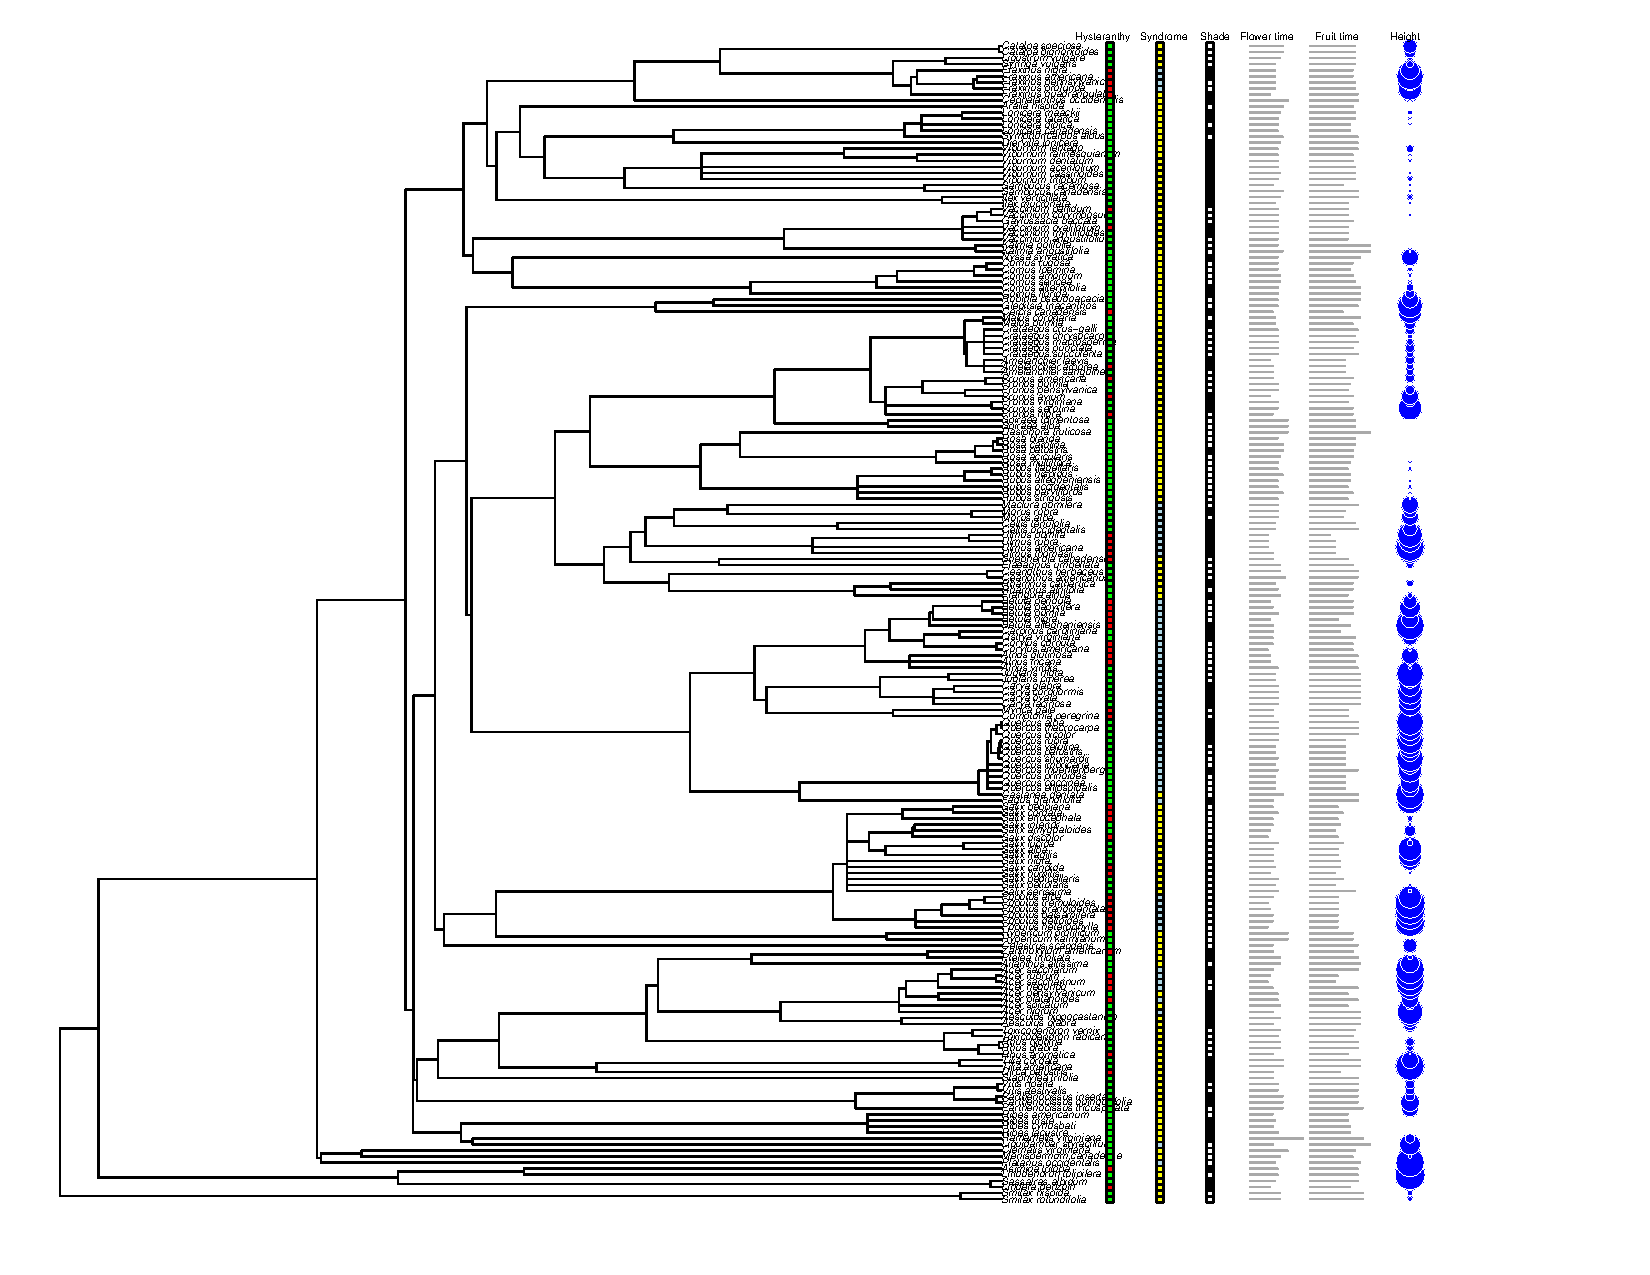
\includegraphics[width=21cm, height=15cm]{tree_full_mich.pdf}\\
\caption{Phylogeny and trait map for Michigan data}
\end{figure}

\begin{figure}[h!]
\begin{knitrout}
\definecolor{shadecolor}{rgb}{0.969, 0.969, 0.969}\color{fgcolor}
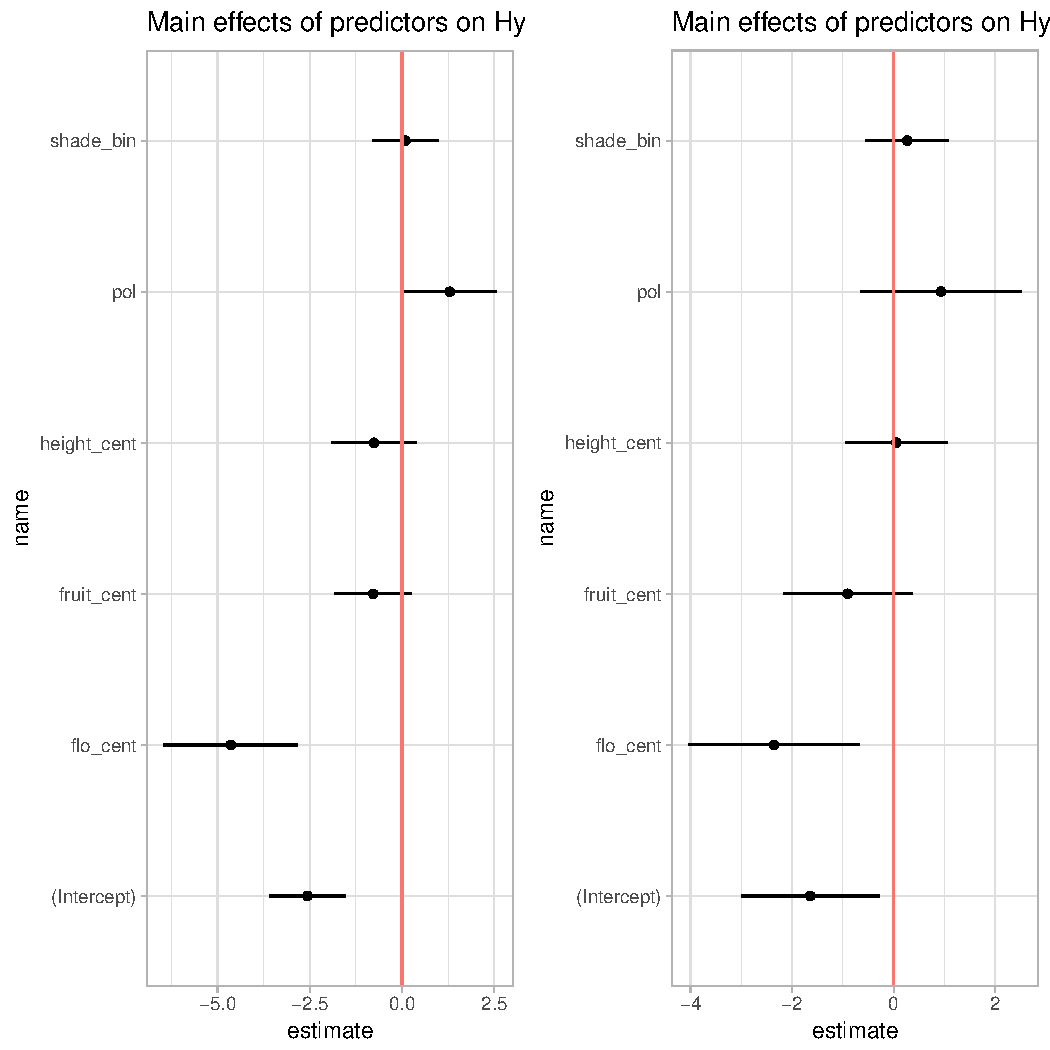
\includegraphics[width=\maxwidth]{figure/unnamed-chunk-5-1} 

\end{knitrout}
\caption{Trait effect sizes}
\end{figure}


\begin{figure}[h!]
\begin{knitrout}
\definecolor{shadecolor}{rgb}{0.969, 0.969, 0.969}\color{fgcolor}
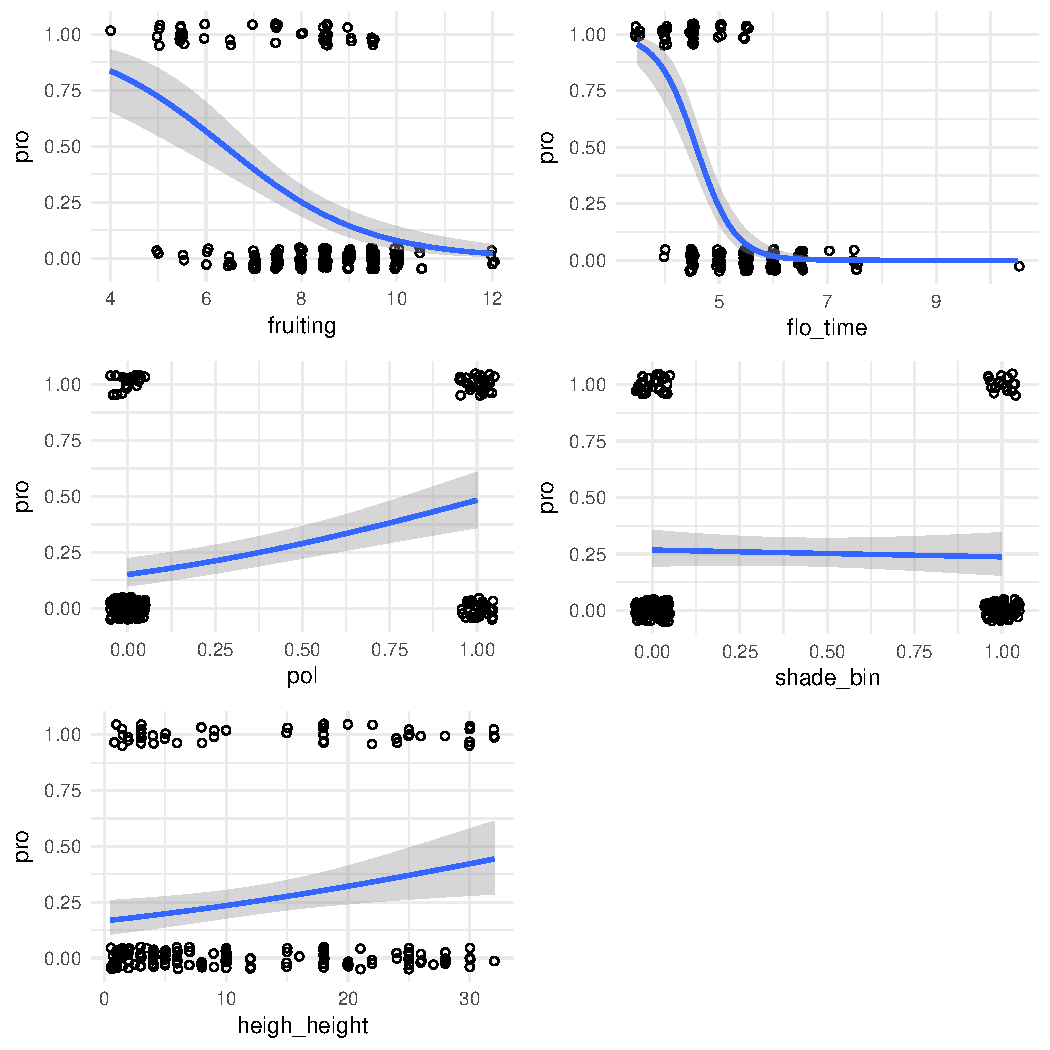
\includegraphics[width=\maxwidth]{figure/unnamed-chunk-6-1} 

\end{knitrout}
\caption{Michigan binomial plots}
\end{figure}

\begin{figure}[h!]
\begin{knitrout}
\definecolor{shadecolor}{rgb}{0.969, 0.969, 0.969}\color{fgcolor}
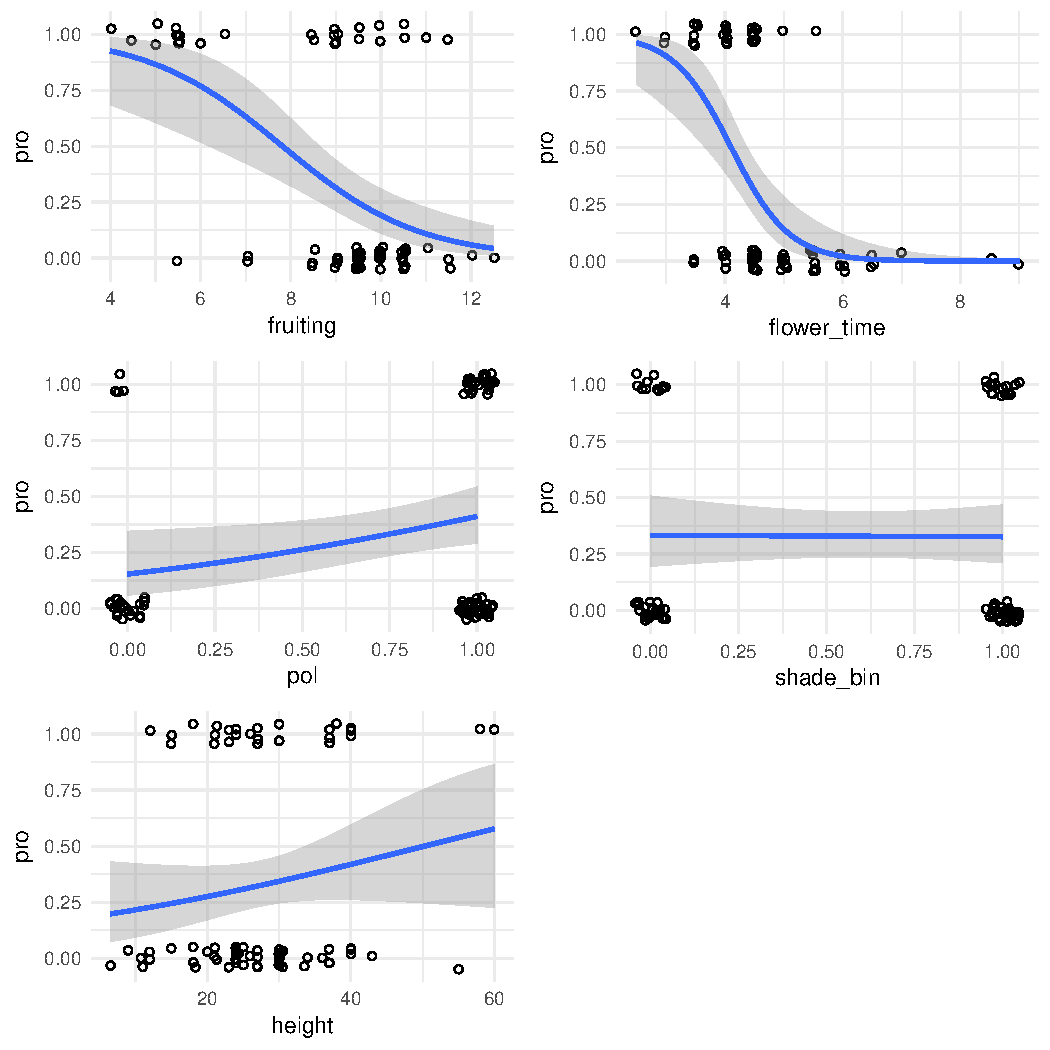
\includegraphics[width=\maxwidth]{figure/unnamed-chunk-7-1} 

\end{knitrout}
\caption{Silvics binomial plots}
\end{figure}

\end{document}
